\documentclass[aps,prb,twocolumn,superscriptaddress,floatfix,longbibliography,citeautoscript]{revtex4-2}

% Conveniently, the citeautoscript option in the revtex4-2 class toggles the spacing & punctuation automatically for superscript vs. bracketed citations. Place citations as if they were in [].
% Uncomment the line below to do superscript citations.
% \setcitestyle{super}

\usepackage{amsmath,amssymb} % math symbols
\usepackage{bm} % bold math font
\usepackage{graphicx} % for figures
\usepackage{comment} % allows block comments
\usepackage[normalem]{ulem} % allows strikeout text, e.g. \sout{text}

% \usepackage{minted} % allows colored code
% \usepackage{textcomp} % This package gives the text quote '

\usepackage{enumitem}
\setlist{noitemsep,leftmargin=*,topsep=0pt,parsep=0pt}

\usepackage{xcolor} % \textcolor{red}{text} will be red for notes
\definecolor{lightgray}{gray}{0.6}
\definecolor{medgray}{gray}{0.4}
\definecolor{mRed}{RGB}{230, 0, 50}
\colorlet{newtextColor}{mRed}

\usepackage{hyperref}
\hypersetup{
colorlinks=true,
urlcolor= blue,
citecolor=blue,
linkcolor= blue,
}

% Code to add paragraph numbers and titles
\newif\ifptitle
\newif\ifpnumber
\newcounter{para}
\newcommand\ptitle[1]{\par\refstepcounter{para}
{\ifpnumber{\noindent\textcolor{lightgray}{\textbf{\thepara}}\indent}\fi}
{\ifptitle{\textbf{[{#1}]}}\fi}}
%\ptitletrue  % comment this line to hide paragraph titles
%\pnumbertrue  % comment this line to hide paragraph numbers

% Code for reviewer text
%\newcommand{\revtext}[1]{\textcolor{reviewColor}{#1}}
\newcommand{\revtext}[1]{\textit{#1}}

% Code to track changes
\newif\iftrackchanges
\newcommand{\newtext}[1]
    {\textcolor{\iftrackchanges newtextColor\else black\fi}{#1}}
\newcommand{\deltext}[1]
    {\iftrackchanges{\textcolor{newtextColor}{\sout{#1}}}\fi}
%\trackchangestrue  % comment to hide tracked changes

% Instead of making TONS of colored newtext, let's just put a colored line next to big blocks of new text.
\usepackage{mdframed}
\newmdenv[
  linecolor={\iftrackchanges newtextColor\else white\fi},
  linewidth=2pt,
  topline=false,
  bottomline=false,
  rightline=false,
  skipabove=\topsep,
  skipbelow=\topsep,
  leftmargin=-12pt,
  innertopmargin=0pt,
  innerbottommargin=0pt
]{newtextblock}

% Uncomment this line if you prefer your vectors to appear as bold letters.
% By default they will appear with arrows over them.
% \renewcommand{\vec}[1]{\bm{#1}}

% Command to mark text in blue/red and define common units
\newcommand{\blue}[1]{\textcolor{blue}{#1}}
\newcommand{\red}[1]{\textcolor{red}{#1}}
\newcommand{\df}[1]{\dfrac}
\newcommand{\mic}{\mu\mathrm{m}}
\newcommand{\nm}{\mathrm{nm}}
\newcommand{\mm}{\mathrm{mm}}
\newcommand{\mrm}[1]{\mathrm{#1}}
\newcommand{\la}{\langle}
\newcommand{\ra}{\rangle}

\ptitletrue
\pnumbertrue

% Replace minted with listings if you don't want to install Pygments
\usepackage{listings}
\usepackage{graphicx}
\usepackage{siunitx}
\usepackage{float}
% minimum font size for figures
\newcommand{\minfont}{6}

% Author affiliations
\newcommand{\heng}{School of Engineering \& Applied Sciences, Harvard University, Cambridge, Massachusetts 02138, USA}
\newcommand{\hphys}{Department of Physics, Harvard University, Cambridge, Massachusetts 02138, USA}

% Allows rewriting the same title in the supplement
\newcommand{\mytitle}{Muon Lifetime and Mass Experiment First Draft}

\begin{document}

\title{\mytitle}

\author{Adam Pearl}
\email[]{apearl@college.harvard.edu}
\affiliation{\hphys}
\author{Nicholas Lyu}
\email[]{nicholaslyu@college.harvard.edu}
\affiliation{\hphys}
% \affiliation{\heng}

\date{\today}

\begin{abstract}
This paper outlines the design, alignment, and calibration of a single-beam optical tweezer apparatus. 
We aim to trap dielectric spheres in solution and measure the trap depth. 
\end{abstract}

\maketitle

%%%%%%%%%%%%%%%%%%%%%%%%%%%%%%%%%%%%%%%%%%%%%%%%%%%%%%%%%%%%%%%%%%%%%%%%
\section{\label{sec:intro}Introduction}

In this experiment we measure the lifetime of the muon as  well as the muon mass. The first evidence of the muon was reported by Street and Stevenson in 1937 when they noticed an anomalous mass range in the \blue{energy spectra of cosmic rays} \cite{PhysRev.52.1003}. In 1947, Valley and Rossi used a cloud chamber to make the \blue{first} measurement of the muon lifetime \cite{PhysRev.59.223}. In this paper, we recreate these findings by detecting muons generated by cosmic rays using a carbon scintillator detector. The current literature value for the mass of the muon is $105.6583755 \pm 0.0000023$ \si{\mega\eV}; the current literature value for the muon lifetime is $2.1969811 \pm 0.0000022 ms$ \cite{ParticleDataGroup:2024cfk}. 

\red{Expand the history and motivation and what a muon is }

%%%%%%%%%%%%%%%%%%%%%%%%%%%%%%%%%%%%%%%%%%%%%%%%%%%%%%%%%%%%%%%%%%%%%%%%
\section{\label{sec:theory}Theory and Background}

 Cosmic rays continuously enter the earth atmosphere at a flux of order $10^{-2}$\si{\per\centi\metre\squared\per\second\per\steradian}. These cosmic rays - primarily protons or other heavy nuclei - collide with particles in the Earth's upper atmosphere producing hadron showers of pions $\pi$ and kaons $K$ through the strong interaction. Charged kaons and pions subsequently decay into which then decay into muons and muon neutrinos through the channels $\pi^{\pm} \to \mu^{\pm} + \nu_\mu$ and $K^{\pm} \to \mu^{\pm} + \nu_\mu$. Unlike its hardonic predecessors, muons have a long lifetime and a large penetration depth \blue{penetration depth?}, allowing them to reach the earth's surface and even pentrate underground \cite{MuonLifetimeWiki}. Upon interacting with the scintillator's material, muons deposit energy via ionization thereby exciting atoms along their paths. When excited atoms fall back to their ground state they emit light which can then be amplified through a photomultiplier tube and converted into a digital signal. After a characteristic liftime, the muons decay according to a weak process shown in figure ~\ref{fig:mu_decay}, as well as its corresponding antimatter decay. Muons may also decay due to nuclear capture \red{how is this accounted for in our experiment?}. \cite{griffiths2008particles}. We can measure the onset time of the muon decay by measuring the signal induced from the light emitted during the electron ionization process (see section ~\ref{sec:lifetime}). The light is then converted into a voltage response that can used as a measure of the ionizing energy of the electron (see section ~\ref{sec:mass}).

 The interaction strength of weak force at the two interaction vertices is given by the fermi coupling constant, $G_F$ . By Fermi's golden rule, the decay rate is proportional to the square of the amplitude of the process, ie. $\Gamma_\mu \propto \left| M \right|^2 \propto G_F^2$. The exact relation between the muon lifetime and $G_F^2$ is given by 

\begin{equation}
    \tau_\mu = \frac{192\pi^3\hbar^7}{G_F^2m_\mu^5 c^4}
\end{equation}

(Griffiths \cite[Chapter 9, p.~314]{griffiths2008particles}). With our mass and lifetime measurements, we can predict the value of $G_F$ (see section ~\ref{sec:Results}).



 
\begin{figure}
    \centering
    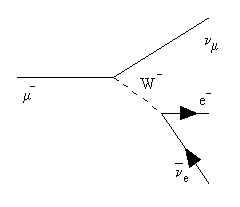
\includegraphics[width=0.5\linewidth]{mudecay.png}
    \caption{Negative muon weak decay channel $\mu \to e^-\Bar{\nu_e}\nu_\mu$.}
    \label{fig:mu_decay}
\end{figure}
 
\subsection{\label{sec:lifetime}Lifetime}
Muons decay exponentially over time. The total number of muons $N$ at a given time $t$ follows the distribution $N(t) = N_0e^{-\Gamma_\mu t}$, where $\Gamma_\mu$ is the muon decay rate. The muon lifetime is then defined as $\tau_\mu = \frac{1}{\Gamma_\mu}$. The muon lifetime can be determined by observing the number of muons that decay at as a function of time $-\dot{N} =\Gamma_\mu N_0e^{-\Gamma_\mu t}$, taking the logarithm of this function and fitting it to a linear model $y(t) = \ln(\Gamma_\mu N_0) - \Gamma_\mu t$.

\subsection{\label{sec:mass}Mass}
In order to measure the muon mass $m_\mu$, we make the important assumtion that the muon decays at rest, meaning that the total energy of the muon is its rest mass, $E_\mu = m_\mu$. The muon decays in a three body decay $\mu \to e^- \nu_\mu \Bar{\nu}_\mu$. The energy carried the electron is then some fraction of the total energy which depends on the relative scattering angles and momenta of the neutrinos. In theory, one could derive the probability density of the electron energy by considering all scattering configurations and use this distribution to fit the experimental electron energy distribution. Instead, we opt to use the highest energy electrons (the maximum of the distribution of $E_e$) in order to estimate $m_\mu$. We do this both for its simplicity and in order to avoid having to model energy losses due to the scintillator's geometry (see appendix). Here we show that the highest energy electrons carry approximately half of the muon rest energy.  

We fix the coordinate frame such that the electron momentum is along the $x$ axis, $\boldsymbol{p_{e}} = (p_e, 0)$. We write the momenta of the neutrinos in terms of generic constants, $\boldsymbol{p_{\Bar{\nu}_e}} = (a, b)$ and $\boldsymbol{p_{{\nu}_\mu}} = (c, d)$. Conservation of momentum along the y axis dictates that $b=-d$, and conservation of momentum in along the x axis dictates that $p_e = -a - c$. Since the neutrinos have (approximately) no rest mass, conservation of energy dictates that, $$E_e + \left| \boldsymbol{p_{\Bar{\nu}_e}}\right| + \left|\boldsymbol{p_{{\nu}_\mu}} \right| = m_\mu \to E_e + \sqrt{a^2 + d^2} + \sqrt{c^2 + d^2} = m_\mu$$. Finally, the energy of the electron can be written as $$E_e = \sqrt{\left|\boldsymbol{p}_e\right|^2 + m_e^2} = \sqrt{p_e^2 + m_e^2} $$

Since $E_e$ only depends on $d$ through equation \blue{number the equations}, we can maximize that equation with respect to $d$ and automatically see that $d = 0$ maximises $E_e$. Taking $d = 0$, the momentum balance reduces to $E_e +a+c = m_\mu$. Substituting this equation into \blue{number the equations} and solving for $E_e$ gives $E_e = \frac{m_\mu}{2} + \frac{m_e^2}{m_\mu}$. In the limit where $ \frac{1}{2} >> m_e^2/m_\mu^2$, the highest energy electrons carry half of the muon's rest mass, $E_e^{\text{max}} \approx m_\mu / 2$. Using the literature values for $m_e$ and $m_\mu$, the ratio $m_e^2/m_\mu^2$ is approximately $10^{-4}$.

With this motivation, we can use the highest energy electrons as a proxy to measure the muon mass. Since our experiment measures voltage rather than energy, we need to be able to convert between output voltage and energy. We do this by running an experiment where we measure the voltages of muons that pass through all three scintillators using a $T\wedge B$ \texttt{START} trigger and $M$ \texttt{STOP} trigger. We make the assumption that a muon that is not stopped by any of the scintillators is minimally ionizing (we address the limitations of this assumption in the discussion session), such that its momentum minimizes the Bethe bloch curve for muons passing through carbon (see section ~\ref{sec:calibration} Since the Bethe Bloche curve is well known, we can use this process to do our conversion \red{improve writing}.

We measure the mass according to the formula

$$m_{\tau} = \frac{2V_e}{V_m}\min\langle \frac{dE}{dx}\rangle_{\mu} \rho h$$

where $V_e$ is the response voltage of the highest energy electrons (see section \blue{results - fitting}), $V_m$ is the mode of the distribution of electron voltages from the minimally ionizing muon measurements, $\langle\frac{dE}{dx}\rangle_{\mu}$ is the minimum of the bethe bloche curve for muons passing through carbon, $\rho$ is the density of the carbon scintillator, and $h$ is the depth of each scintillator.

\blue{values}


\section{\label{sec:setup}Experimental Setup}
\subsection{Detector and instrumentation}
Our experimental apparatus consists primarily of three plastic scintillators, each with the same dimensions, long, flat and thin (length $>$ width $>$ height). The height is measured by ruler to be $2.7 \pm 0.1$ \si{\cm}. The material is polystyrene with an additional phosphor, p-terpheny, responsible for emitting light under ionization. In the subsequent analysis we approximate the material properties as those of carbon, and take the density of the material to be $\rho = 1.08 $ \si{\gram\per\cm\cubed}, approximately half that of graphite \cite{MuonLifetimeWiki}.  The scintillators are connected to photomultiplier tubes (PMTs) at each end which liberate electrons through the photoelectric effect. These electrons are accelerated through a potential and cause an avalanche, thereby amplifiyng the signal by a factor of $10^6$ to $10^8$ \cite{MuonLifetimeWiki}. The signal generated is then passed through processed through LeCroy  fan-outs, discriminators, gates, and delays as described in section ~\ref{sec:triggers} and shown in figure ~\ref{fig:schematic}.


\section{\label{sec:methods}Methods}


\subsection{\label{sec:triggers}Triggers and delays}

For both the mass and lifetime measurements, we look at the small fraction of muons that decay in the middle detector. The signature of these events is that the muons are detected both in the top and middle scintillators; we therefore use a $T\wedge M \wedge \Bar{B}$ \texttt{START} gate. In order to detect emitted electrons, we use a $\Bar{T}\wedge M$ coincidence \texttt{STOP} gate that captures electrons that either stay in the middle detector or exit towards the bottom. We use a coincidence gate rather than a simple $M$ gate for robustness to noise at the cost of having reduced counts.
In order to avoid false \texttt{START} caused by a $T\wedge M\wedge B$ event, we both extend and delay the $B$ pulse. We chose a delay of \red{delay} and a pulse duration of \red{pulse duration}.


\subsection{Fitting and background correction}

 We use a \red{name of software?} program that measures the time difference between the \texttt{START} trigger and \texttt{STOP} triggers. 

\blue{We explain how we fit the logarithmic decay curve, including our assumption of constant background and how we corrected for it, and our method for determining the optimal hyperparameters (clipping data and bin width).} 
\subsection{\label{sec:calibration}Electron pulse calibration}
The Bethe Bloche equation describes how the average rate of ionizing energy loss per unit distance, $-\langle \frac{dE}{dx}\rangle$ changes as a function of the relativistic factor $\beta\gamma$. A particles is referred to as minimally ionizing if it travels at a $\beta \gamma$ that minimizes the Bethe Bloche under the relevant parameters. Muons incident upon the detectors have a wide range of momenta; in order to be able to compare voltage output to an energy, we look to measure the voltage output of minimally ionizing muons whose energy is well known. We do this by choosing a $T \wedge M \wedge B$ trigger under the assumption that muons which are not stopped by the three scintillators are minimally ionizing \blue{this is kinda wack}. Using the height of the detector, we can estimate $E$ for a MIP. We trigger on $TMB$ and measure the average electron pulse height. We compare this to the $E$ to get a conversion from pulse amplitude (voltage) to energy, $V_m$.
\subsection{Error propagation}
The error on the muon lifetime is estimate from the error on the slope of the linear fit to the logarithm of the exponential decay. The standard error on $\tau_\mu$ is given as $\sigma_{\tau_\mu} = \left|\frac{d\Gamma_\mu}{d\tau_\mu}\right|\sigma_{\Gamma_\mu} = \frac{\sigma_{\Gamma_\mu}}{\Gamma_\mu^2}$
 
 
For the mass measurement, the error for the mass will depend on the standard error on the electron pulse amplitude conversion as well the error associated with the energy measurement. We need to think carefully about this since we are measuring the max of a distribution.

We assume variables are independent and use the additive error $$\sigma_{m_{\tau_\mu}} = 2\sqrt{\sigma_{V_e}^2 + \sigma_{\rho}^2 + \sigma_{h}^2}$$ where we neglect the uncertainty on $\min\langle \frac{dE}{dx}\rangle_{\mu}$. The uncertainty on the density of carbon is \blue{check this}. The uncertainty on $h$ is taken to be $0.1$ \si{\cm}, the width of the smallest increment on the ruler used to measure $h$.

\red{error prop for fermi constant.}

\subsection{Instrumentation schematic}
We first run our signals through fan outs, then discriminators, then through delays, coincidence detectors, ect... We include a detailed schematic here.
\begin{figure}
    \centering
    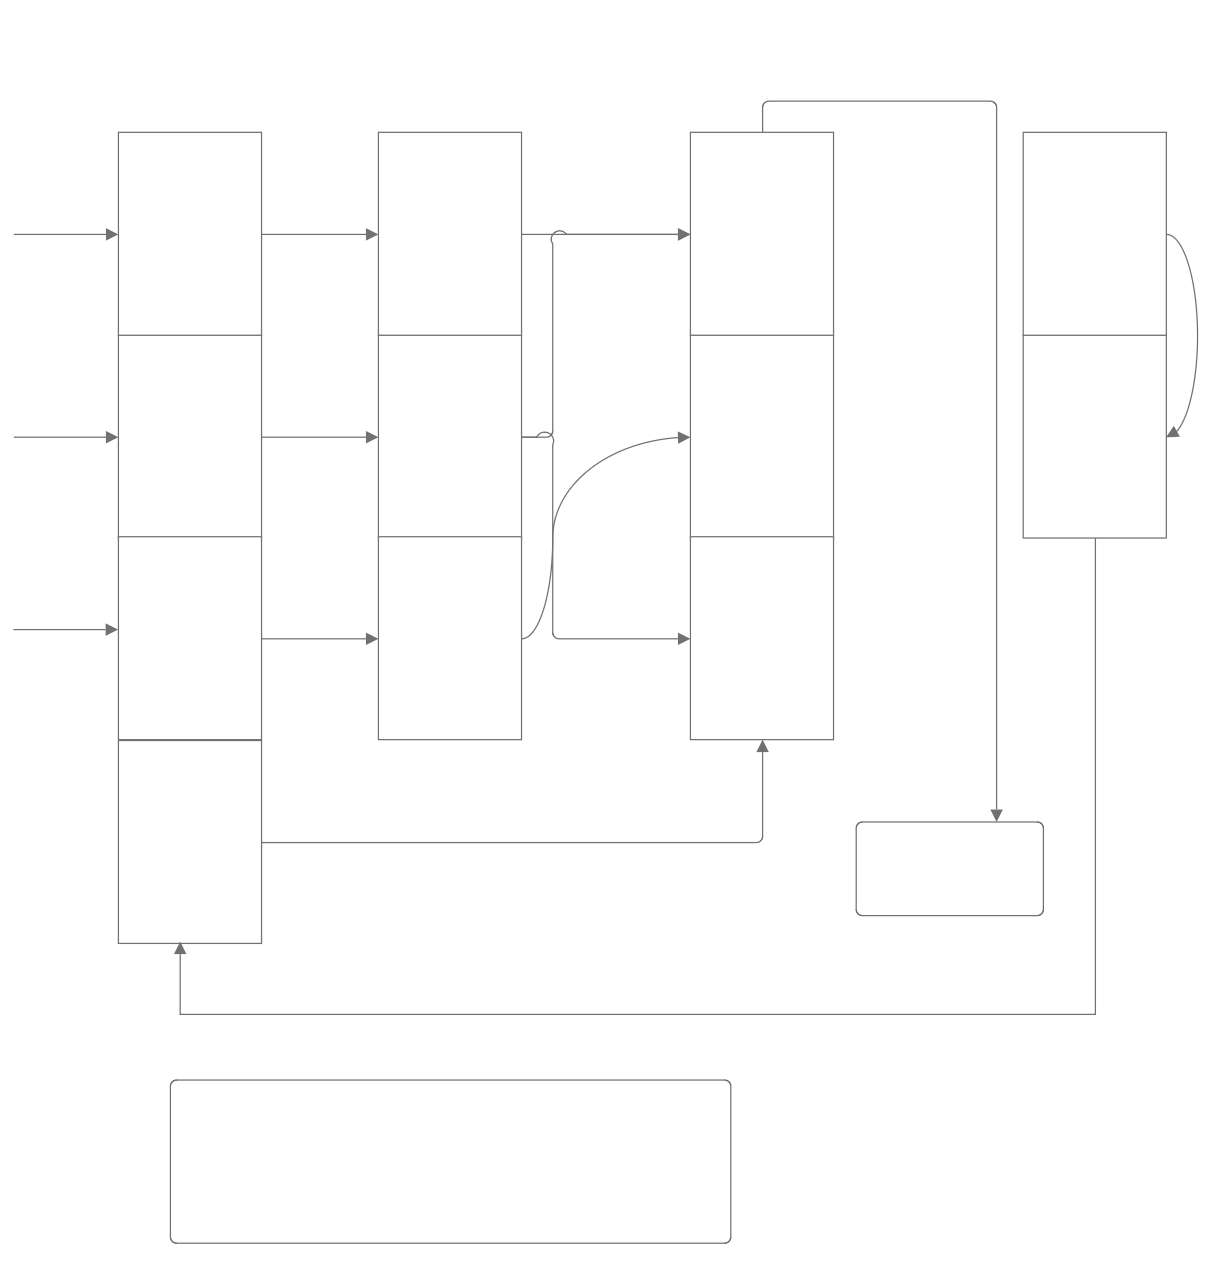
\includegraphics[width=0.5\linewidth]{schematic.png}
    \caption{Placeholder cable schematic}
    \label{fig:schematic}
\end{figure}




\section{\label{sec:Results} Results}
\subsection{Thresholds and efficiency}
%%%%%%%%%%%%%%%%%%%%%%%%%%%%%%%%%%%%%%%%%%%%%%%%%%%%%%%%%%%%%%%%%%%%%%%%

\begin{acknowledgments}
\end{acknowledgments}

\bibliographystyle{apsrev4-2}
\bibliography{refs} % Include the bibliography file

\end{document}